\documentclass[12pt,draftcls,onecolumn]{IEEEtran}
%\documentclass[onecolumn]{IEEEtran}

\usepackage{amsmath}
\usepackage{amsthm}
\usepackage{amssymb}  % assumes amsmath package installed
%\usepackage{algorithmic}
%\usepackage{algorithm}
\usepackage{algorithm}
\usepackage{algpseudocode}
\usepackage{algpseudocode}

\algnewcommand{\algorithmicand}{\textbf{ and }}
\algnewcommand{\algorithmicor}{\textbf{ or }}
\algnewcommand{\OR}{\algorithmicor}
\algnewcommand{\AND}{\algorithmicand}
\algnewcommand{\var}{\texttt}

\usepackage{cite}
\usepackage{color}
\usepackage{comment}
\usepackage{epsfig}
\usepackage{float}
\usepackage{graphicx}
\usepackage{multicol}
\usepackage{subfigure}
\usepackage{setspace}
\usepackage{comment}
\usepackage{subfig} % for subfigures
\usepackage{caption}

%\usepackage[linesnumbered,ruled]{algorithm2e}

\usepackage[none]{hyphenat}

\newtheorem{theorem}{Theorem}[section]
\newtheorem{lemma}[theorem]{Lemma}
\newtheorem{proposition}[theorem]{Proposition}
\newtheorem{corollary}[theorem]{Corollary}
\newtheorem{remark}[theorem]{remark}

\begin{document}

\title{Path Planning of Webot Satisficing Experiment ----  Milestones Generation}


\author{  Min Zheng \\  \today}

\date{\today}

% make the title area
\maketitle


%\IEEEpeerreviewmaketitle

%%%%%%%%%%%%%%%%%%%%%%%%%%%%%%%%%%%%%%%%%%%%%%%%%%%%%%%%%%%%%%%%%%%%%%%%%%%%%%
The project considers the integrated navigation and control of an unmanned ground vehicle(UGV) deployed to visually classify multiple targets in an obstacle-populated environment. 
This report discusses the hybrid sampling method to obtain milestones for the roadmap. 

\section{Probelm setup and previous results} 

The weBot workspace and two-dimensional representation constructed in MatLab are shown in the figure below  (Figure \ref{fig:2}). 


\begin{figure}[p]
\centering
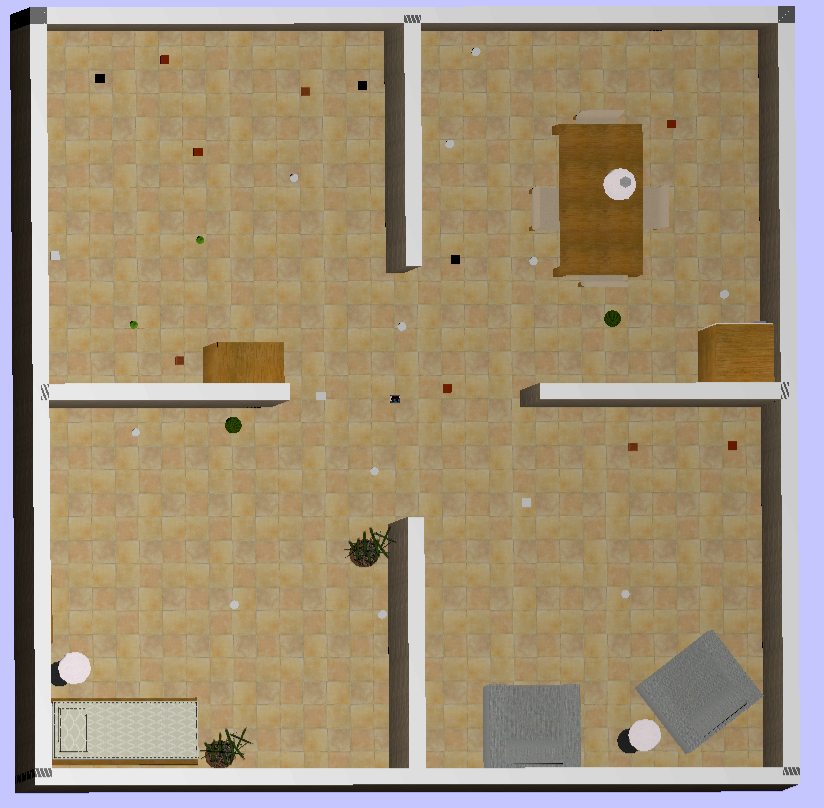
\includegraphics[width=10cm]{figures/webotTop}
  \caption{Top view of the webot environment}
  \label{fig:1}
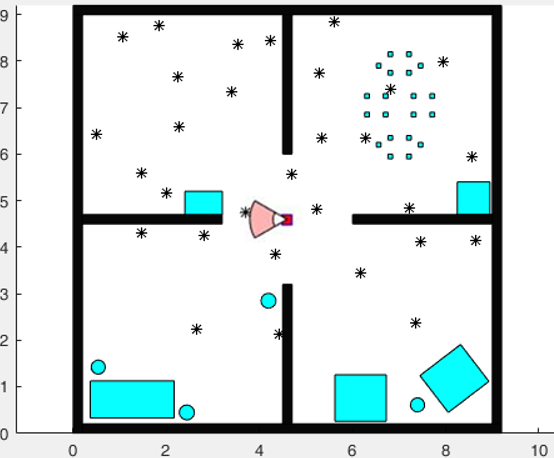
\includegraphics[width=13cm]{figures/newWorld}
  \caption{2D representation built in MatLab. Obstacles are represented by colored regions, and targets represented by the stars. The UGV is  the red square, while its FOV is the red area within the fan shape.}
  \label{fig:2}
\end{figure}


EER method is applied in the milestone generation and the on-line path planning, so that the UGV finds and interacts with the targets motivated by the entropy reduction of revealing a possible feature. 
The target features, Bayesian Network(BN) structure and Conditional Probability Table(CPT) are the same as the one used in human tests as well as visual classification.
The targets have 3 levels of features: shape, color and textures, each is a random variable named $X_{1}$, $X_{2}$ and $X_{3}$.
By the EER calculation(in Report 170724), given the CPTs shown in Table \ref{table.1}, the corresponding EER is shown in  Figure \ref{fig:13} and  Figure \ref{fig:14}.

\begin{table}[!htbp]
\centering
\caption{An example of CPT of the target objects}
\label{table.1}
\begin{tabular}{|l|l|l|l|l|l|l|l|l|} % l = left, r = right, c = center
\hline
Cue & \multicolumn{8}{c|}{P(cue)} \\ \hline % l = left, r = right, c = center
$x_{k1}$ & \multicolumn{4}{c|}{0.43 (sphere)} & \multicolumn{4}{c|}{0.57 (box)} \\ \hline % l = left, r = right, c = center
$x_{k2}$ & \multicolumn{2}{c|}{0.64} & \multicolumn{2}{c|}{0.36} & \multicolumn{2}{c|}{0.69} & \multicolumn{2}{c|}{0.31} \\ \hline % l = left, r = right, c = center
$x_{k3}$ & \multicolumn{1}{c|}{0.69} & \multicolumn{1}{c|}{0.31} & \multicolumn{1}{c|}{0.37} & \multicolumn{1}{c|}{0.63} & \multicolumn{1}{c|}{0.08} & \multicolumn{1}{c|}{0.92} & \multicolumn{1}{c|}{0.21} & \multicolumn{1}{c|}{0.79} \\ \hline
$ID$ & Apple & Watermelon & Orange & Basketball & Cardboard box & Wooden box & Computer & Book \\ \hline
$Z$ &  \multicolumn{1}{c|}{0.9} &  \multicolumn{1}{c|}{0.1} & \multicolumn{1}{c|}{0.9}  & \multicolumn{1}{c|}{0.9}  &\multicolumn{1} {c|}{0.9}  & \multicolumn{1}{c|}{0.9}   &\multicolumn{1}{c|}{0.9}  &\multicolumn{1} {c|}{0.9}   \\ \hline % l = left, r = right, c = center
\end{tabular}
\end{table}


\clearpage





\begin{figure}
 \centering
  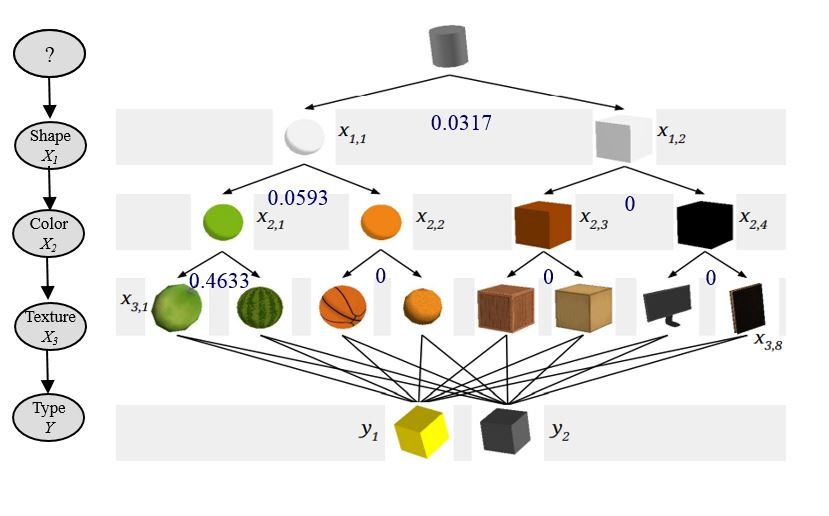
\includegraphics[width=15cm]{figures/oneStepEER}
  \caption{Single-step EER}
  \label{fig:13}
\end{figure}

\begin{figure}
 \centering
  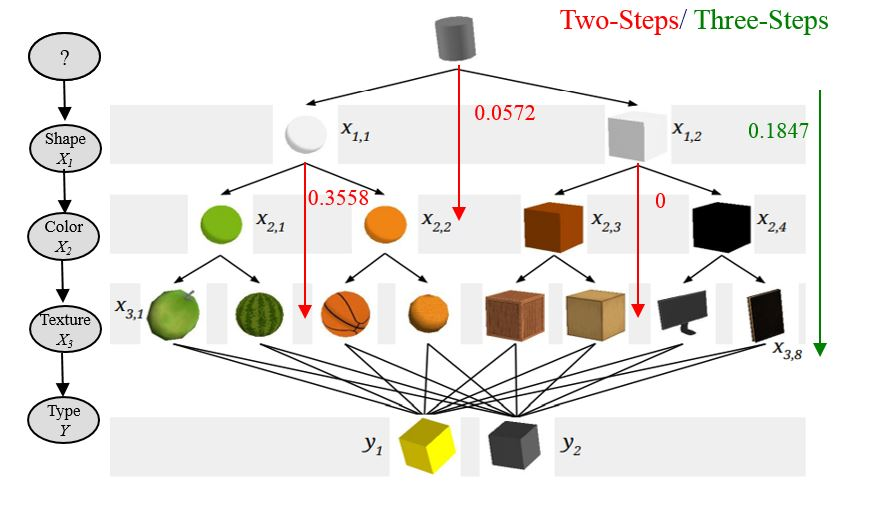
\includegraphics[width=15cm]{figures/someStepEER}
  \caption{Multiple-steps EER}
  \label{fig:14}
\end{figure}


\clearpage
%%%%%%%%%%%%%%%%%%%%%%%%%%%%%%%%%%%%%%%%%%%%%%%%%%%%%%%%%%%%%%%%%%%%%%%%%%%%%%
\section{Milestones Sampling}
The minimum resolution required for the roadmap is 200x200 in 2D space. 
Therefore a simplified sampling method is proposed (Algorithm 1).
A hybrid strategy is used to combine a bridge test for narrow passages and a uniform probability density function in wide-open regions in order to provide coverage in both.
Let $b$ and $b'$ be two random variables representing the two endpoints of a bridge in $C_{2D}$.
While $C_{2D}$ is configuration in 2D space,  $q \equiv [x  \quad  y  ]^T$.


\subsection{RBB Sampling}
Since bridges must connect $C_{obstacles}$, $b$ is sampled from a uniform distribution $f(b)$ over $CB$.
And $b'$ is sampled from a multivariate Gaussian PDF that is radially symmetric, with mean at $b$'s location, and a self-defined standard deviation.

%\begin{equation}
%f(b'\; |\; b) = \lambda_{b}(b')I(b')/Z_{b}
%  \label{eq:2}
%  \end{equation}
%Where $/Z_{b}$ is the normalization factor, and 


Let $N_{H}$ denote the total number of milestones generated using hybrid strategy.
We assign a user-defined parameter $0\leq v \leq 1$, which emphasizes either either distribution in the mixture.
So that the $N_{H}$  milestones should be split into  $N_{U} =N_{H}*v $ and $N_{RBB} =N_{H}*(1-v) $, representing uniform and RBB (Randomized Bridge Builder).

As discussed in the Narrow Passage Sampling paper, RBB may generate some milestones near the corner, which is unhelpful.
To reduce the false positives near corner, the orthogonal test is performed for a RBB generated milestone. 
The test draws a line segment orthogonal to the bridge.
The line segment length is a pre-defined variable.
The milestone is accepted if the line segment is collision-free with the $CB$.
 Figure \ref{fig:15} and  Figure \ref{fig:16} demonstrates an example case of using the orthogonal test.


\begin{figure*}[htp]
  \centering
  \subfigure[Example case, the orthogonal test is not used. Some milestones are generated near the corner, which is not helpful.]{\includegraphics[width=12cm]{figures//RBB_woOrthoTest}}\quad
  \subfigure[Example case of applying the orthogonal test ]{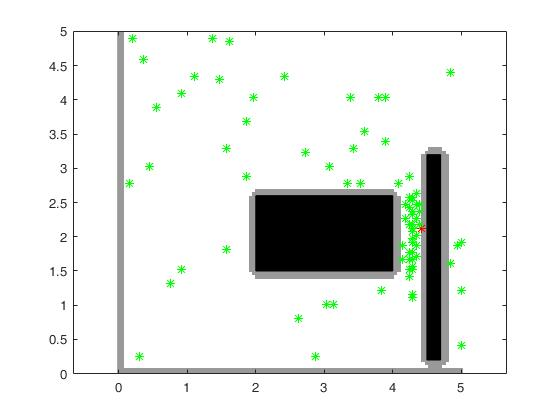
\includegraphics[width=12cm]{figures/RBB_wOrthoTest}}\quad
  \caption{An example case on the orthogonal test}
  \label{fig:15}
\end{figure*}


%\begin{equation}
%\pi_{H} = v\pi_{G}+(1-v)\pi_{U}
%  \label{eq:1}
%  \end{equation}
\begin{algorithm}
   \caption{Simplified Hybrid Sampling Combined with EER}
    \begin{algorithmic}[1]
      \Function{Milestones}{$C$, $C_{free}$}\Comment{Where MS - milestone}
        \State Let $N_{Unif}$, $N_{RBB}$, $N_{EER}$ be the number of milestones desired
        \While {$N_{U}$ not reached \OR  $N_{RBB}$ not reached}
            \State Uniformly generate a point $q_1$ in $C_{2D}$  
	 \If  {$q_1 \in C_{free}$ \AND $N_{U}$ not reached}
	 \State Record $q_1$
	 \Else
	  \While {$q_p$ is not a valid RBB milestone}
             \State Generate $q_2$ by multivariate Gaussian PDF
	  \If { $q_2 \in CB$}
	  \State $q_p = (q_1+q_2)/2$	
	  \If {$q_p \in C_{free}$ \AND  Orthogonal Test Passes}
	  \State Record $q_p$
	  \EndIf 	
             \EndIf 
	 \EndWhile	 
	 \EndIf
        \EndWhile
        \While {$N_{EER}$ not reached}
        \State Calculate $EER(q)$ 
        \EndWhile
      
       \EndFunction
\end{algorithmic}
\end{algorithm}

\clearpage



%\begin{figure}
% \centering
%  \includegraphics[width=12cm]{figures/RBB_woOrthoTest}
%  \caption{}
%  \label{fig:15}
%\end{figure}
%
%\begin{figure}
% \centering
%  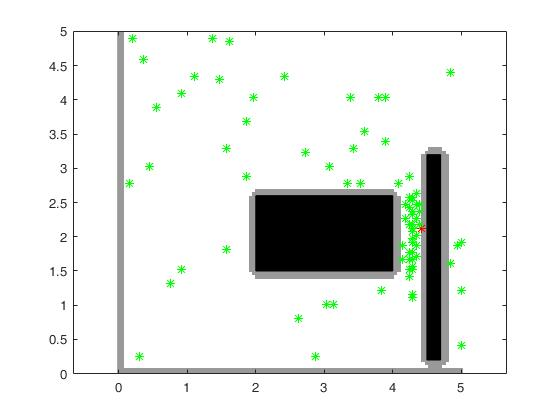
\includegraphics[width=12cm]{figures/RBB_wOrthoTest}
%  \caption{Example case of applying the orthogonal test.}
%  \label{fig:16}
%\end{figure}



When calculating the EER of a given target, if the configuration is in $\mathcal{C}_{Target}$, its EER is the single-step EER of the nearest target if there is cue unrevealed. 
Currently, only single-step EER is considered, because multiple-step EER is rather complex.
 For example, if two targets are both in the FOV, and the nearest one has only one cue to be revealed, the robot may be able to reveal cues of the second target without changing configuration.
A zoom-in example with target A and B (Figure \ref{fig:17}) demonstrates a case with the proposed protocol.
Even though milestone a and b are near A, they are not in the  $\mathcal{C}_{Target}$ region of target A. 
Therefore their EER is the EER of target B.
Milestone c and d are in the $\mathcal{C}_{Target}$ of both A and B. 
Since they are nearer to target A, their EER is that of A.



The milestone generated for the entire road-map is shown in\ref{fig:16}. 
A possible plan is to select, for example 50 milestones that have the highest EER. 
Then another 50 milestones is randomly selected from the rest. 
Meanwhile, the given the 2D configuration of a milestone, the third dimension $\theta$ can be determined either from reading the pre-calculated result or re-calculating by the method in Section $\mathcal{C}_{Target}$.


\begin{figure}
 \centering
  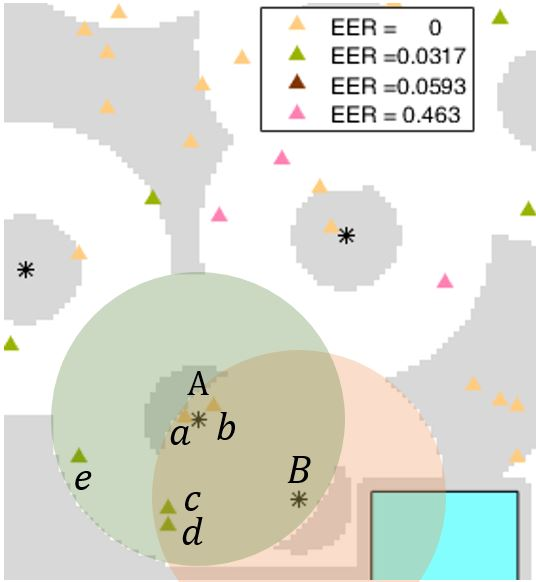
\includegraphics[width=8cm]{figures/EER_zoom}
  \caption{Zoom in of an example of milestones, where the green and orange circles represent the regions that the target A and B can be observed correspondingly. a-e are the generated milestones.}
  \label{fig:17}
\end{figure}


\begin{figure}
 \centering
  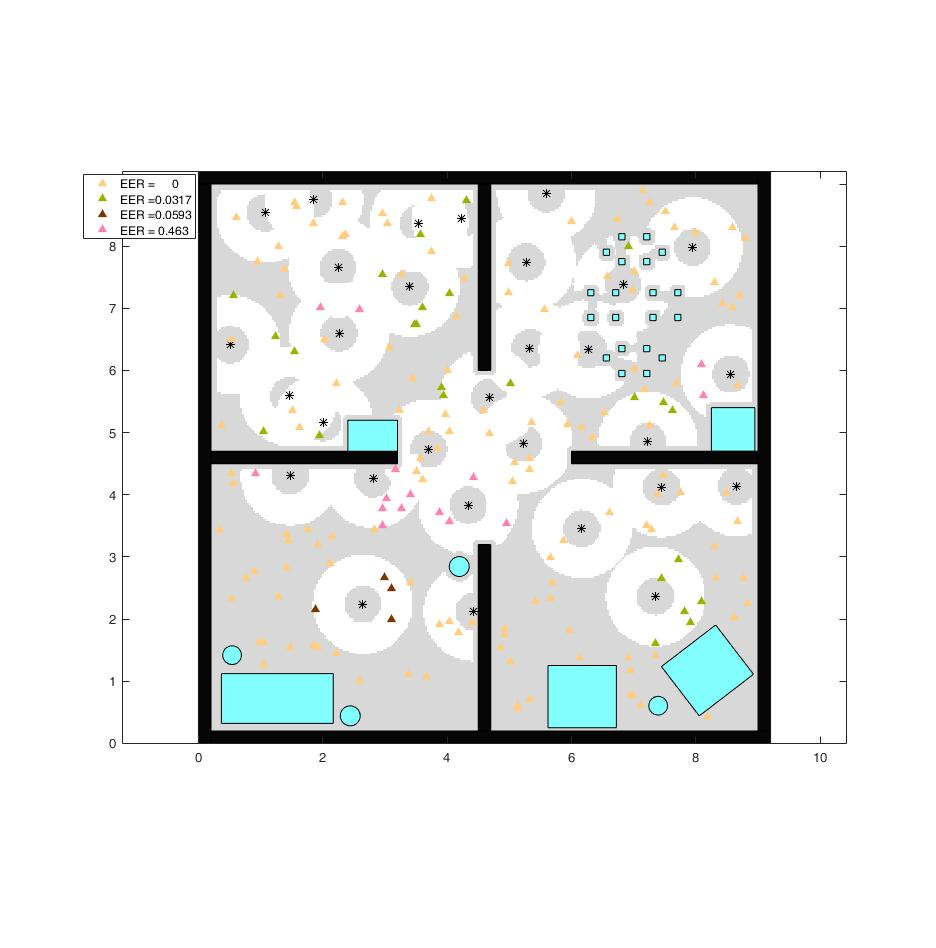
\includegraphics[width=20cm]{figures/milestone180}
  \caption{Example of sampling 180 milestones}
  \label{fig:16}
\end{figure}


\clearpage
%%%%%%%%%%%%%%%%%%%%%%%%%%%%%%%%%%%%%%%%%%%%%%%%%%%%%%%%%%%%%%%%%%%%%%%%%%%%%%
\section{Milestones connectivity}
A 2-D connectivity array is constructed.
For any pair of two milestones, their distance is stored in the array if they are connected, otherwise it is recorded as infinity.
Two milestones are connected if the line segment connecting the two does not collide with any obstacle, and the length of the line segment is less than a user-defined threshold. 
An example of connectivity for 50 milestones is shown in Figure \ref{fig:18}.

\begin{figure}
 \centering
  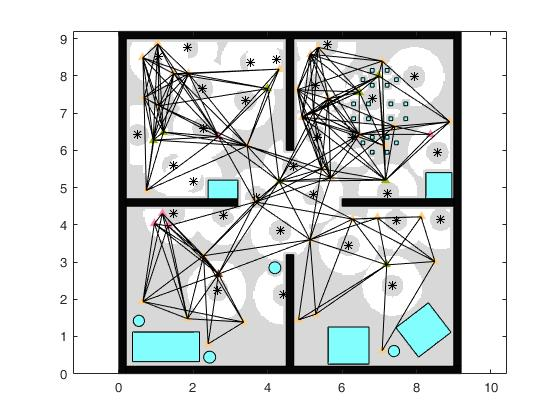
\includegraphics[width=18cm]{figures/connect50MS}
  \caption{Example of connectivity of 50 milestones, while max distance of connectivity is 3.}
  \label{fig:18}
\end{figure}
\end{document}
